\providecommand{\main}{..}
\documentclass[\main/master.tex]{subfiles}
\begin{document}
\chapter{theoretical background}\label{chp:example-2}
\section{devices}
\subsection{arduino}


\section{Arduino}
Arduino is an open-source microcontroller board project used for building low cost and simple digital devices and circuits. Each microcontroller contains a microprocessor, controller, serial communication interface and is equipped with digital and analog input/output pins. The microcontrollers are controlled using C and C++ programming languages, and could be operated as stand alone or connected to the computer through serial communication. 
\par
There are multiple Arduino board models, we would focus on Arduino Mega 2560. The Arduino Mega 2560 is based on the ATmega2560, an Atmel 8-bit AVR controller. Also the board has 54 digital input/output pins of which 15 could be used as PWM outputs and a 16 MHz crystal oscillator (clock). In reality the arduino doesn't have analog output, to modulate the output Pulse Width Modulation technique is used.
\par
The controller is switching on/off the signal between the full Vcc of the board and off (5-0[V]), generating a square wave. The duration of time signal on is called the pulse width. The controller is able to modulate the pulse width, and change the ratio of time signal is on compare to off. The voltage is determined by the ratio of the time voltage is on compare to time voltage off, which is called duty cycle. 100\% duty cycle means the power is always on, 0\% duty cycle power is always off and 50\% duty cycle signal is on and off in equal times. 
\\
\\
\par

\begin{figure}[htbp]
	\centering
	\fbox{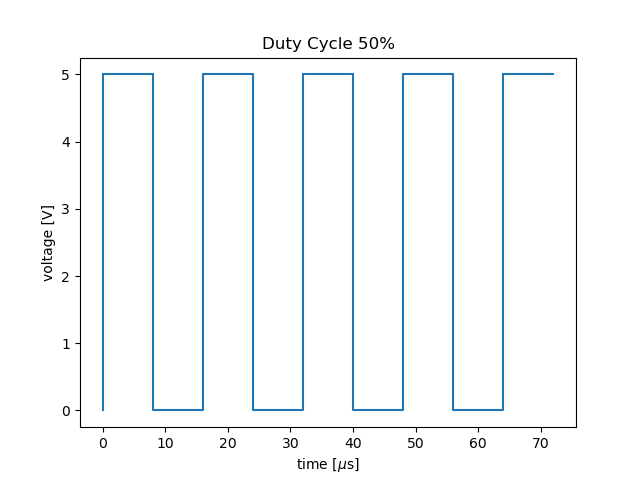
\includegraphics[scale=0.5]{\main/images/devices/duty50.png}}
	\caption[duty cycle 50\%]{50\% duty cycle  - signal is on and off equal times}
	\label{fig:duty50}
\end{figure}
Repeating that pattern fast enough results in an analog signal as if the signal is a steady voltage. This method is able to generate signals between the full Vcc of the board and off. The signal resolution is limited by the microcontroller resolution (8-bit). Due to the fast clock the of the arduino - the PWM frequency is about 500Hz.
\par
\begin{figure}[htbp]
	\centering
	\fbox{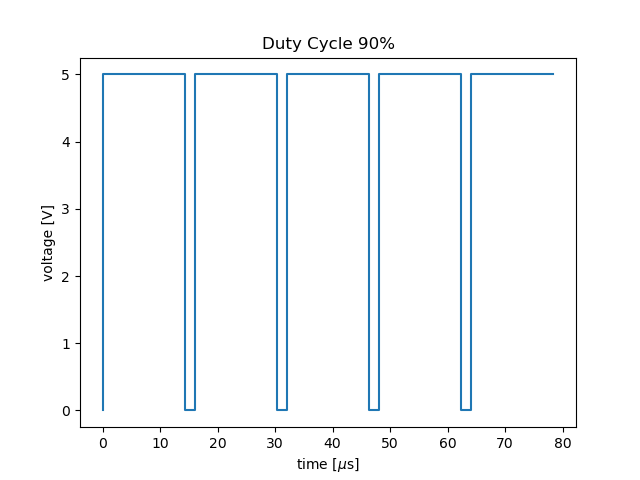
\includegraphics[scale=0.5]{\main/images/devices/duty90.png}}
	\caption[duty cycle 90\%]{90\% of the time signal on, equivalamt to 90\% of the full Vcc signal}
	\label{fig:duty90}
\end{figure}


\par
Using this method with a led connected, the led brightness could be controlled at about 2ms speed. Since the clock is connected to all PWM pins, if they all are in the same duty cycle, they are in sync. All pins are having a changing voltage, but they all have the same voltage, alowing to connect them in series and increase the output current, and the LED power. In conclusion this is a real-time controlled, fast-modulated, high power light source. 



\subsection{light guide}
\color{blue}
\par
Light guides are used to distribute light from the source to a particular area that requires illumination. They are made up of a transparent material (glass or plastic) and thin filaments and are capable of transmitting light signals though internal reflections.  

Light pipe technology utilizes clear plastic tubes that transmit light from a light source. There are two basic styles of LED light pipes – rigid and flexible - and both are capable of redirecting light with minimal loss of concentration.
\color{black}


\subsection{Light Emitting Diode (LED)}
The light emitting diode (led) is a high power long lifetime light source semiconductor based. The led is emitting light when current flows through it, the light power is propotional to the current. Led could be modulated at up to 100MHz, fast compare to the experiment. The emitted light is incoherent in width meaning it's hard to focus it to a point (not diffraction limited). The emitted light is incoherent in length causing wide band spectrum, although spectrum is sufficiently narrow to appear as a pure color to the human eye.
\par

The working principle is a semiconductor p-n junction with forward voltage causing recombination of electrons with holes. The recombination is releasing energy in form of spontanious emmission photons. 
\par
\color{blue}
\par
\color{black}


\subsection{laser}
\subsection{aom}
\section{vacuum theory}
\section{torsion theory}
\section{optical cooling}
\section{pid}
\section{accuracy}
\doublespacing
\hspace{5 mm} This another example chapter with a working reference as see in Chapter~\ref{chp:example-1}. There I also made an example of an equation, see Eqn.~\ref{eqn:energy-mass-equivalence-relation}. We also created an example image, see Fig.~\ref{fig:sine-wave}.
\begin{figure}[htbp]
	\centering
	\fbox{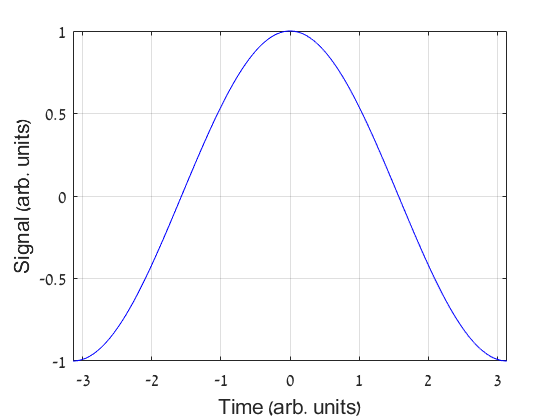
\includegraphics[scale=0.75]{\main/images/chapter_2_example/img_example_2.png}}
	\caption[Another Example Image]{Another Example Image. This image is also labeled internally so we can referenc it throughout the text.}
	\label{fig:cosine-wave}
\end{figure}
\end{document}